\section{Parsing Vue.js}

\subsection{Assumptions}
It is assumed that the Vue.js code for which interaction diagrams are going to be generated compiles and does not contain syntactical errors. Naturally, logical errors are not an issue.
\subsection{Limitations}
\label{concept:parsing_limits}

In order to be able to generate interaction diagrams, which capture every aspect of Vue.js, the generation must be based on an \gls{ast}, which covers every possible syntax, such as \cite{eslint_vue_parser_ast}. The approach proposed here only includes the following features of Vue.js:
\begin{itemize}
    \item Event handlers (including anonymous method syntax and method reference syntax)
    \item Any one or two-way binding expressions (\code{v-model}, \code{v-bind}, "moustache", \code{v-if}) excluding \code{v-else}
    \item \code{v-for} statements for lists, excluding iterating through properties of an object or iteration with index (property zipped with index)
    \item Computed properties
    \item Complex objects
    \item Non-nested lists 
    \item Methods, including the resolution of arguments, they have been called with (excluding other methods as arguments)
\end{itemize}
\newpage
\subsection{AST}
\label{ast}
\begin{lstlisting}[language=antrl,basicstyle=\fontsize{8}{8}\selectfont\ttfamily]
grammar vue_simple;

program: bindings methodDefinitions createdMethod topLevelProperties computedProperties;

topLevelProperties: thisIdentifier*;
methodDefinitions: methodDefinition*; 
createdMethod: methodDefinition;
computedProperties: (methodDefinitionIdentifier reads writes calls)*;

methodDefinition: methodDefinitionIdentifier methodArgs reads writes calls;

methodArgs: NAME_IDENTIFIER*;
reads: accessedVariable*;
writes: accessedVariable*;
calls: calledMethod*;

calledMethod: calledMethodIdentifier '(' calledArgs ')';
accessedVariable: identifier;
calledArgs: (calledMethod | accessedVariable)*;

bindings: binding*;
binding: tag bindingSource+;
bindingSource: (accessedVariable | calledMethod) (EVENT_BINDING | ONE_WAY_BINDING) | accessedVariable TWO_WAY_BINDING;

tag: name tagId loc;
tagId: LINE '_' COLUMN '_' LINE '_' COLUMN;
name: UNICODE | identifier;
loc: start end;
start: LINE COLUMN;
end: LINE COLUMN;

calledMethodIdentifier: methodDefinitionIdentifier | id* NAME_IDENTIFIER;

methodDefinitionIdentifier: THIS NAME_IDENTIFIER;
thisIdentifier: THIS identifier;
identifier: NAME_IDENTIFIER id*;

id: NUMERIC_INDEX | GENERIC_INDEX | NAME_IDENTIFIER;

//terminals, tokens
LINE: [0-9]+;
COLUMN: [0-9]+;

EVENT_BINDING: 'event';
TWO_WAY_BINDING: 'two-way';
ONE_WAY_BINDING: 'one-way';

GENERIC_INDEX: 'i' | 'j' | 'k' | 'l' | 'm' | 'n';
THIS: 'this';

NUMERIC_INDEX: [0-9]+;
NAME_IDENTIFIER:  JS_IDENTIFIER;
JS_IDENTIFIER:  (UNICODE | '$' | '_') (UNICODE | '$' | '_' | [0-9])*;
UNICODE: [\u0000-\uFFFF];
\end{lstlisting}


A Vue.js \gls{spa}, including all the necessary information for \ref{concept:parsing_limits}, can be defined using the above grammar. The application consists of \astnode{bindings} \astnode{methodDefinitions} a \astnode{createdMethod}, \astnode{topLevelProperties} and \astnode{computedProperties}. 

The top level properties (\astnode{topLevelProperties}) represent the \code{data} object of the Vue.js \code{script} tag. Each property will be represented as a list of identifiers and prefixed with \astnode{THIS}, in order to indicate it belongs to the model. Objects are represented flattened, e.g. \code{problem:\{a:0, b:0\}} will be represented as follows:

\begin{figure}[H]
    \centering
    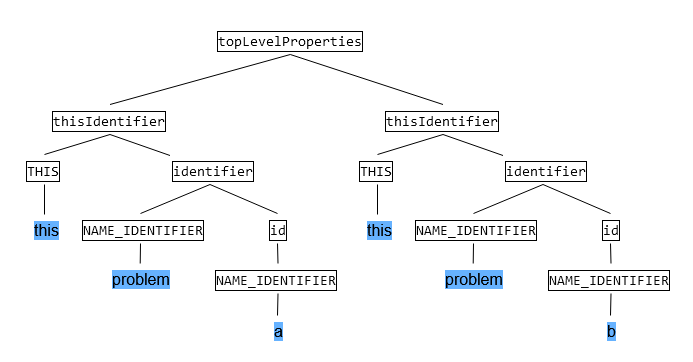
\includegraphics[width=0.8\textwidth]{images/ast_top_level.png}
     \caption{\gls{ast} for top-level properties example }
     \label{fig:ast_top_level}
\end{figure}

Bindings of the Vue.js component (\astnode{bindings}) can be obtained from the \code{template}. Each binding consists of an HTML tag, a list of binding sources for that tag (pairs of variable or method calls) and a binding type. The binding type is represented as one of event (\astnode{EVENT_BINDING}), one-way (\astnode{ONE_WAY_BINDING}) or two-way (\astnode{TWO_WAY_BINDING}). Two-way bindings are only valid with properties, whereas for events and one-way bindings, both method calls and properties are possible. This is the case since in Vue.js a binding source could be an expressions defined as an inline anonymous functions, e.g.
\code{<div v-if=\"value === true && func()\"/>}
. The binding sources are a list, since a tag could have multiple different bound properties, or a bound expression. The information about how exactly the properties are bound, if it is the same type of binding, is discarded.

Method calls (\astnode{calledMethod}) include the arguments they have been called with - other methods or just variables. It is also possible to call methods with binary expressions. Those are represented as a special method, which takes 2 arguments - the left and right side operators of the binary expression. Expressions with multiple terms can be represented as multiple binary expressions. This method representation loses information such as the order of operations, but since we are only interested in which properties are being accessed, this loss does not pose an issue.

A special case is accessing lists. For example \code{<div v-bind="problems[0].a"/>} would result in the following \gls{ast}:

\begin{figure}[H]
    \centering
    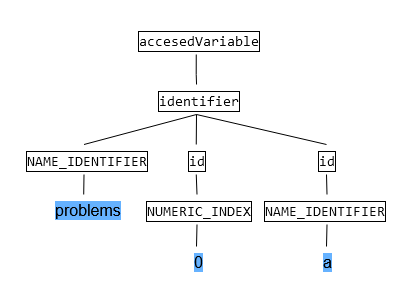
\includegraphics[width=0.7\textwidth]{images/ast_problems_0_a.png}
     \caption{\gls{ast} for a list access example }
     \label{fig:ast_list_simple}
\end{figure}
Another special case are \code{v-for} statements, which are substituted. The list
\begin{lstlisting}[style=html]
<ul>
  <li v-for="subject in subjects" :key="subject.id">
    {{ subject.problems[0] }}
  </li>
</ul>
\end{lstlisting}
would result in \code{subjects[i].problems[0]}, which in term produces the below \gls{ast}:

\begin{figure}[H]
    \centering
    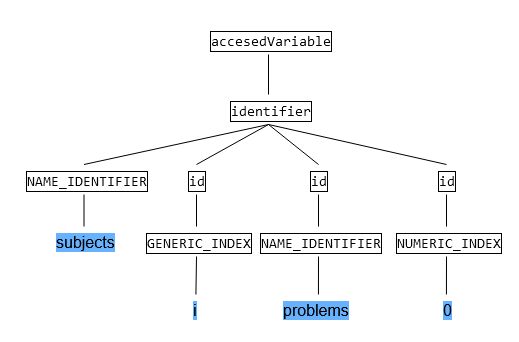
\includegraphics[width=0.7\textwidth]{images/ast_numeric_generic.png}
     \caption{\gls{ast} for a \code{v-for} substitution example }
     \label{fig:ast_list_complex}
\end{figure}

Each \astnode{tag} includes its location in the source code (starting and ending line and column), which can also be used as an identifier. Tags also have humanly readable names, which are either equal to the text of the tag, if it exists, or to the identifier of the first binding. 

All methods, from in the \code{method} object of the view-model, are included in \astnode{methodDefinitions}. Each of them consists of the following:
\begin{itemize}
    \item \astnode{identifier} - an identifier, equal to \astnode{THIS} followed by the name of the method
    \item \astnode{arguments} - names of arguments, each of which is a simple name identifiers
    \item \astnode{reads} - variable it reads from
    \item \astnode{writes} - variables it writes to
    \item \astnode{calls} - method calls, including arguments, same as for bindings 
\end{itemize}

Computed properties (\astnode{computedProperties}) are similar to \astnode{methodDefinitions} with the exception that they do not have arguments. Albeit bad practice, it is still possible for computed properties to have side effects and therefore they were modelled as methods.

%%%%%%%%%%%%%%%%%%%%%%%%%%%%%%%%%%%%%
%                                   %
%   Interaction Diagram Generation  %
%                                   %
%%%%%%%%%%%%%%%%%%%%%%%%%%%%%%%%%%%%%
\section{Interaction Diagram Generation}

The simplified Vue.js \gls{ast} \ref{ast} can be used to create a directed graph, which will represent the interaction diagrams. It is hard to directly generate this graph for lists, therefore the capabilities of a directed, compound graph will be leveraged and later on converted to a directed graph. 
The core idea of the algorithm is to generate vertices only for nodes which are being accessed,instead of the whole application and connect them based on their identifiers. A second pass of the data is required in order to add additional edges for lists. In this section the term node will always be used to refer to a \gls{ast} node of the simplified Vue.js \gls{ast} \ref{ast} and vertex always refers to vertices in the interaction diagram graph, in order to avoid confusion.

Vertices in this graph will have the following properties:
\label{concept:interaction_diagram_structure}
\begin{enumerate}
    \item \gls{guid} - used to reference and globally identify the vertex.
    \item \code{label} - the name of the vertex, which is going to be displayed.
    \item \code{type} - the type of the vertex (data, tag or method). Additionally for data vertices: numeric, generic or undefined (representing simple data vertices).
    \item \code{loc} - defined only on tag vertices. Their location in the source code.
    \item \code{parent} - defined only on vertices of type 'data'. A \gls{guid} of another vertex, used for a child/parent relationship (compound graph).
\end{enumerate}

Edges in the graph are directed and each have a label property, which is one of 'event', 'calls' or 'simple'. 

\subsection{Variable Identifiers}
\label{concept:variable_identifiers}
Variable identifiers are represented by \astnode{identifier} and \astnode{thisIdentifier} in the \gls{ast} \ref{ast}. For the \astnode{THIS} node and for each \astnode{id} node in the \astnode{identifier} or \astnode{thisIdentifier} a vertex is created in order. 
Those vertices are connected using unidirectional edges, labeled with 'simple' and also each vertex (excluding the first one) has its parent set to the previous in the chain. There is one exception to this process - when written to from a method (\astnode{write}), nodes of type \astnode{GENERIC_INDEX} are omitted. The reason behind this will be explained in \ref{concept:why_create_list};

Each vertex has a \gls{guid} equal to the value of its terminal symbols - \astnode{NUMERIC_INDEX}, \astnode{GENERIC_INDEX} or \astnode{NAME_IDENTIFIER}, concatenated with the value of the previous vertex.
The \code{label} of those vertices are equal to the terminal symbol for \astnode{NAME_IDENTIFIER} nodes. For \astnode{GENERIC_INDEX} and \astnode{NUMERIC_INDEX} nodes, the \code{label} is obtained by enclosing it with square brackets and concatenating it with the \code{label} of the previous vertex. Set the type of each vertex to 'data'. Add the type 'numeric' to vertices created from \astnode{NUMERIC_INDEX} nodes and 'generic' to vertices created from \astnode{GENERIC_INDEX} nodes. 

\begin{figure}[H]
    \centering
    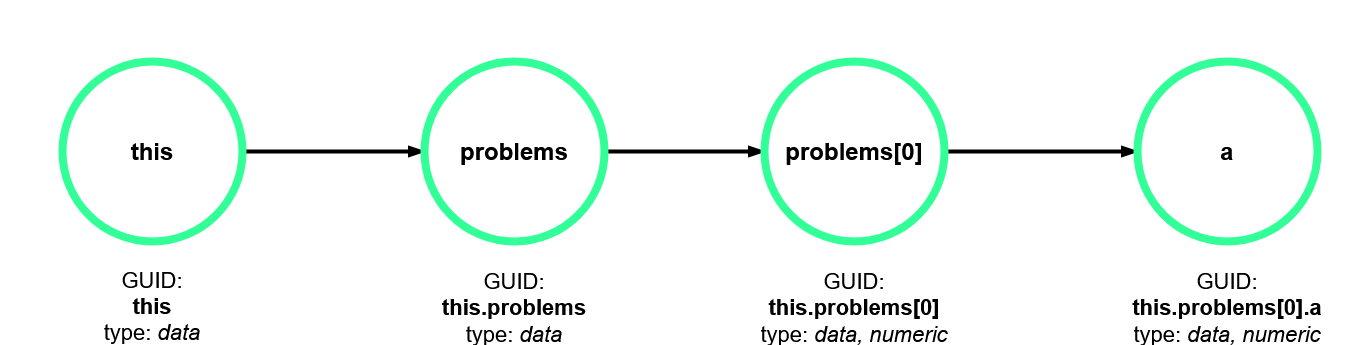
\includegraphics[width=0.65\textwidth]{images/graph_simple.png}
     \caption{Example Graph obtained for the identifier \code{this.problems[0].a} }
     \label{fig:graph_simple}
\end{figure}

\subsection{Object representation}
Using the representation for identifiers in the previous section, objects will result in being displayed dynamically, based on which of their properties are accessed. Nodes and edges are created on a 'create if non-existent' basis, e.g. if \code{this.problem.b} is accessed after \code{this.problem.a} in \ref{fig:graph_object} it will only result in the creation of the node \code{b} and edge \code{this.problem} $\rightarrow$  \code{this.problem.b}.

\begin{figure}[H]
    \centering
    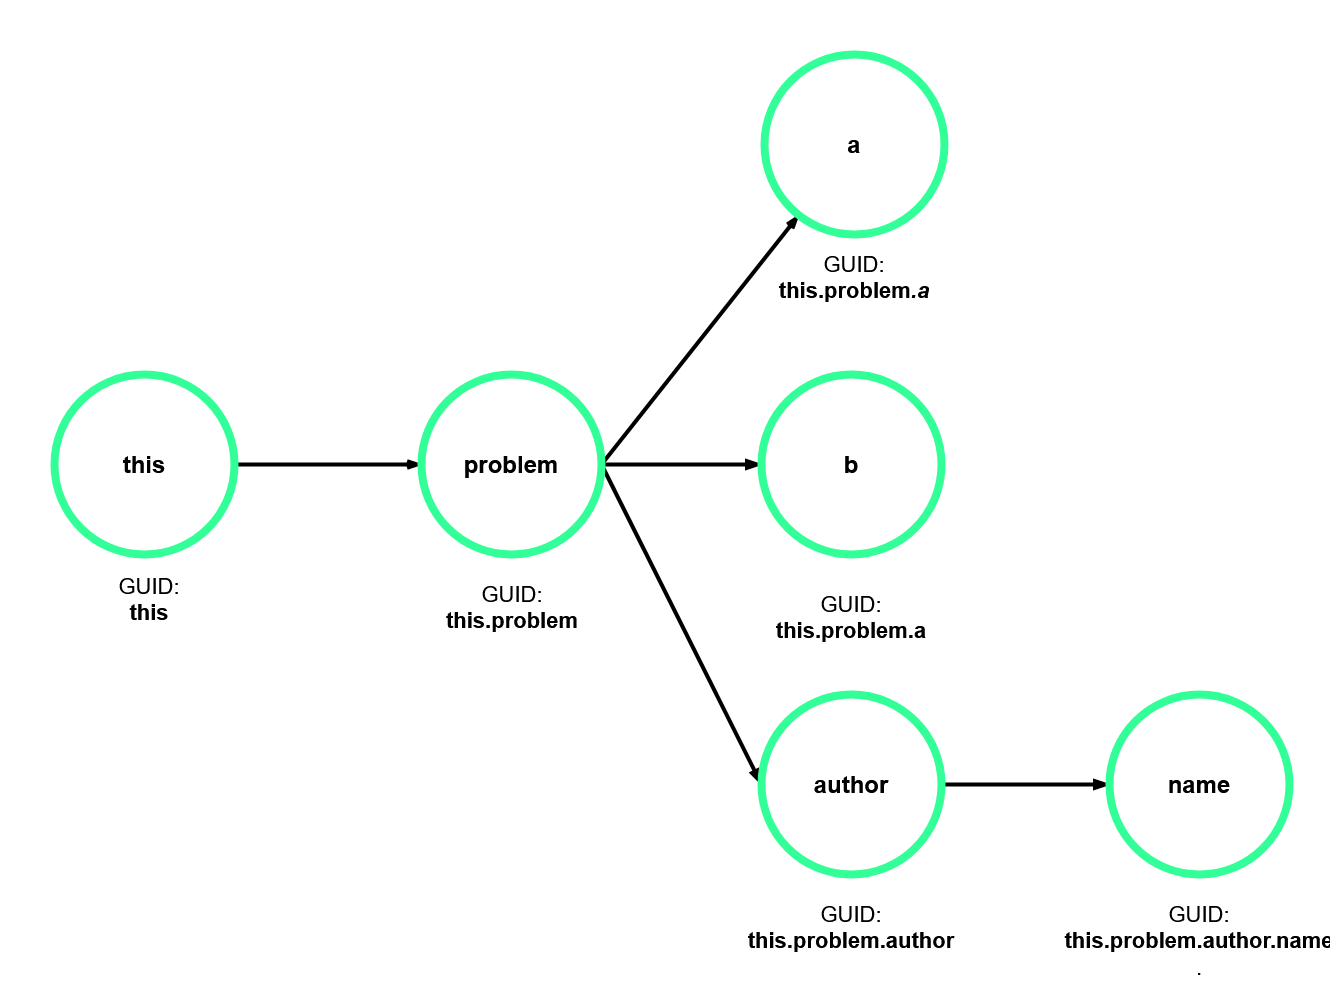
\includegraphics[width=0.7\textwidth]{images/graph_object.png}
     \caption{Example generated graph for object property accesses \code{this.problem.a}, \code{this.problem.b},  \code{this.problem.author.name} }
     \label{fig:graph_object}
\end{figure}

Updates can be formulated nicely with the above representation. If \code{problem} were to be changed, it would result in a cascade update of all of its properties. If \code{author} would change, it would only result in a cascading change in \code{name}. 

\subsection{List representation}
Fig. \ref{fig:graph_complete_example} shows the abstract idea behind list representations.
Concrete list elements, which are accessed, are denoted as $P_{<index>}$ and additionally a vertex $P_{all}$, which can be used to update all elements of a list\label{concept:why_create_list} and their properties, is created.
Another vertex $P_{any}$ is also created, which can be used to observe once any vertex of $P_1$, $P_2$, $P_3$, \dots $P_n$ changes. 

If $P_1$ were to be updated by any method, it would not result in updates to any of $P_2$, $P_3$, \dots $P_n$, however in an update to $P_{any}$.
 The same construct can also be leveraged when it comes to properties of list elements.
 Each top level property of that element will have an $all$ vertex, connected to the $P_{all}$ node of the list. An example of this can be seen in the upcoming section \ref{fig:graph_complete_example}.  

\label{concept:list_creation}
\begin{figure}[H]
    \centering
    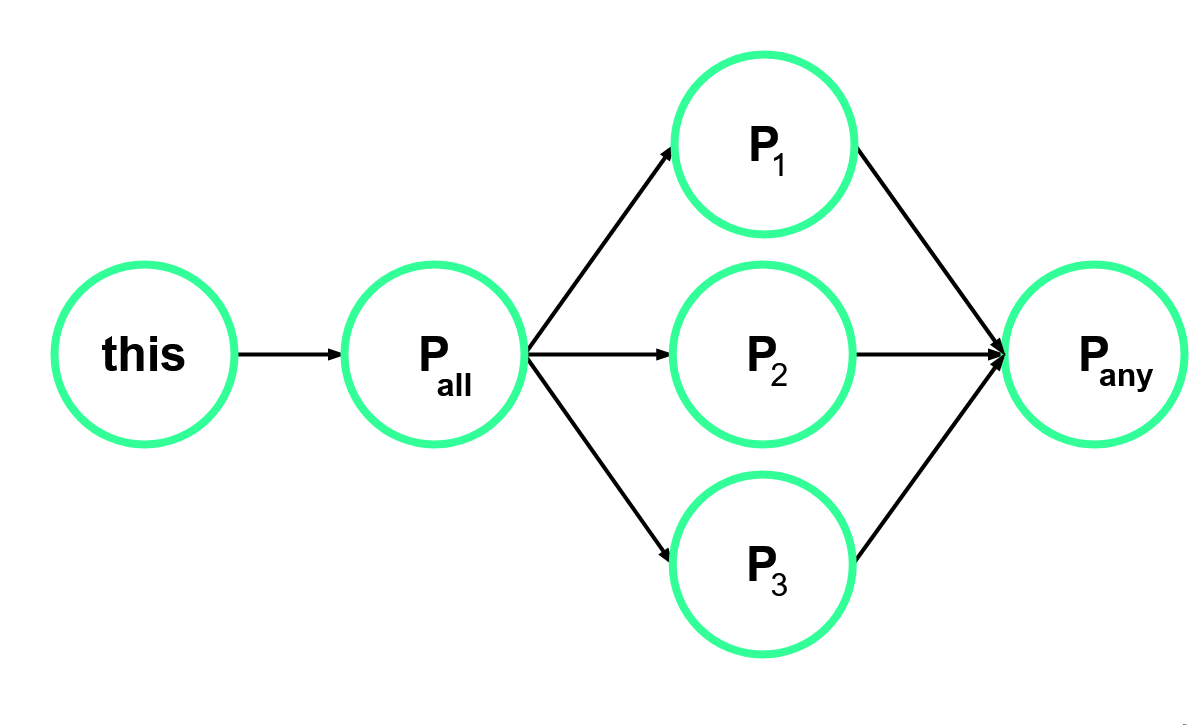
\includegraphics[width=0.65\textwidth]{images/graph_list_generic.png}
     \caption{Abstract list representation}
     \label{fig:graph_list_generic}
\end{figure}

\begin{figure}[H]
    \centering
    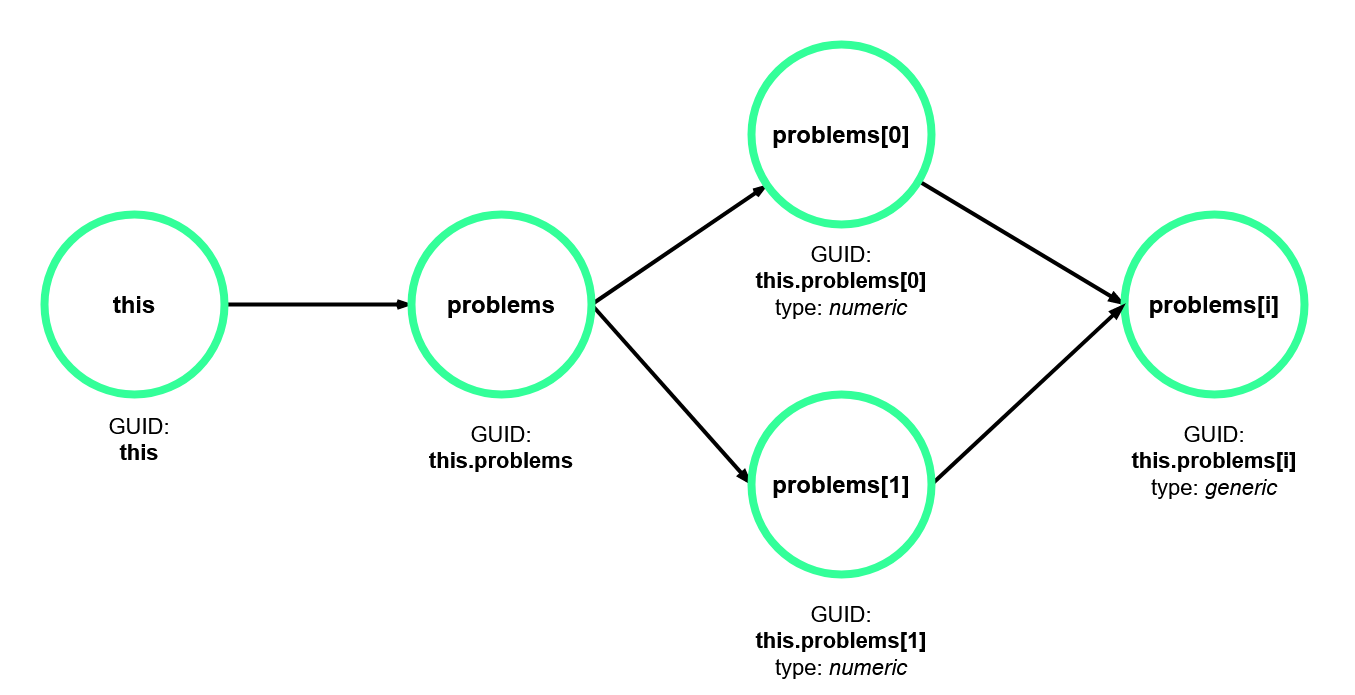
\includegraphics[width=0.7\textwidth]{images/graph_list.png}
     \caption{Concrete example of a list representation}
     \label{fig:graph_list}
\end{figure}

\subsection{Method representation}
\label{concept:methods}
Methods have two related \gls{ast} nodes - \astnode{methodDefinition}, representing the definition of a method and \astnode{calledMethod} representing the concrete call of a method, including parameters. 

\subsubsection{Vertex for Method}
First it should be determined if a vertex needs to be created for a \astnode{calledMethod} node. Only vertices for methods belonging to the context are created. This can be determined by looking up the name of the \astnode{calledMethod} in \astnode{methodDefinition}, ignoring \astnode{THIS}. If the lookup is successful a vertex should be created as described below. If not, it should be checked if the method is a method call on a top level property instance(e.g. \code{this.problems.push()}). This can be done by comparing if it starts in the same way as one of \code{topLevelProperties}.
If that's the case, it is assumed, that it mutates whole property and the method should instead be treated as a write operation.
If both of the above fail, the called method does not belong to context and is of no interest.

The next step is to resolve the names of the arguments it has been called with - \astnode{calledArgs}. Every argument, that can neither be found in \astnode{computedProperties} nor \astnode{topLevelProperties} is replace by a fixed string such as \textit{OTHER} or \textit{*}. In order to obtain the \gls{guid} of the vertex, the name of the \astnode{methodDefinitionIdentifier} is taken, \astnode{THIS} is excluded, and concatenated with the resolved arguments, which are joined with commas  and surrounded with brackets. The \code{label} of this node is equal to its name, excluding \astnode{THIS} the from arguments.

The vertex for the method call is now completed. Multiple calls of this method with the same arguments will all point to this same vertex.

\subsubsection{Vertices for nodes it interacts with}
Now vertices for nodes the method interacts with, based on its \astnode{methodDefinition}, have to be created. Those include the variables it reads - \astnode{reads}, writes - \astnode{writes} and methods it calls - \astnode{calls}. 

Firstly, the arguments from the \astnode{methodDefinition} need to be substituted with the resolved arguments the method was actually called with for all \astnode{reads}, \astnode{writes}  \astnode{calls} referencing them. Now all, which do not start with \astnode{THIS} can be discarded, since they do not belong to the context. 

Once filtered out, create a list of vertices for each variable in \astnode{reads} and \astnode{writes} as described in \ref{concept:variable_identifiers} and connect the most precise of those (the last of each list) to the method vertex. For vertices resulting from \astnode{writes}, this edge has a label of 'writes' ,the property vertex as source and method vertex as sink. For vertices resulting from \astnode{reads}, this edge has the method vertex as source and property vertex as sink. 
Finally the process described in this section (\ref{concept:methods}) is repeated recursively for each \astnode{calledMethod} node in \astnode{calls} and an edge labeled 'calls' is added from the current method vertex to the resulting ones. 

\subsection{Computed Property representation}
\label{concept:computed_property}

Computed properties are represented similarly to methods, except they cannot have arguments, so no substitution of arguments is required. When defining their \code{label} and \gls{guid} both are equal to the \astnode{methodDefinitionIdentifier}. \astnode{reads}, \astnode{writes} and \astnode{calls} are computed in the same manner as methods \ref{concept:algorithm_create_diagrams}. 

\subsection{Generating Interactions}
\label{concept:algorithm_create_diagrams}
\begin{figure}[H]
    \centering
    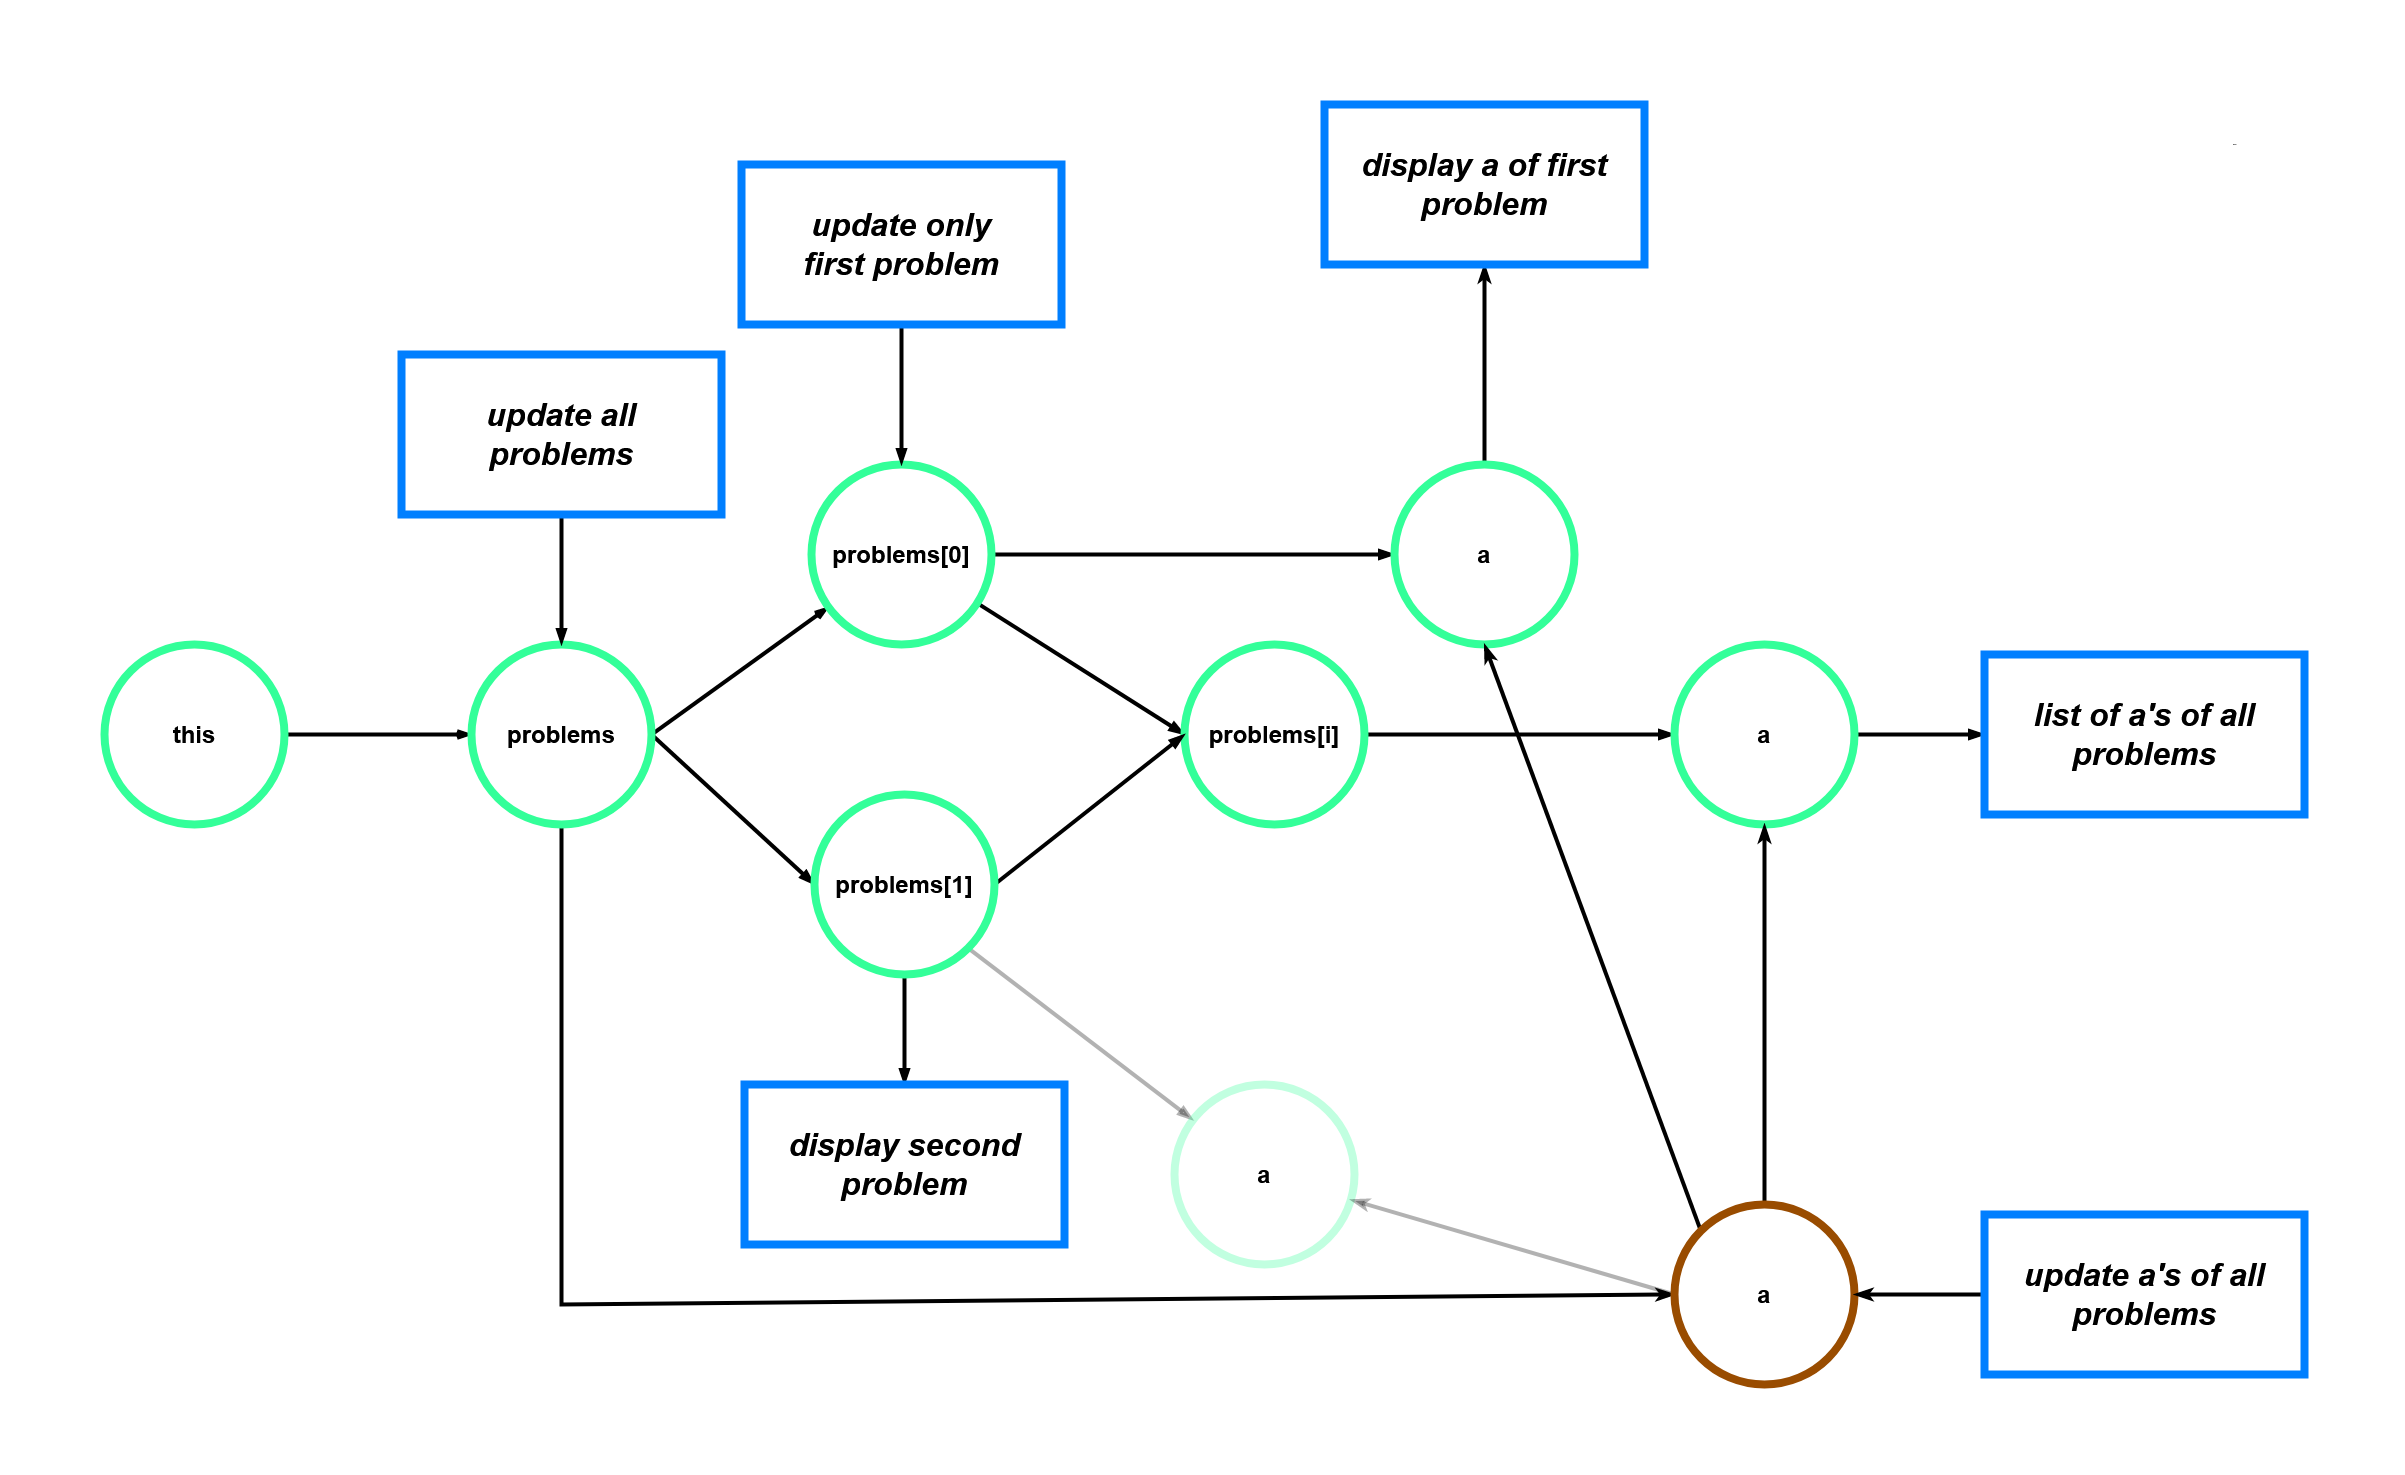
\includegraphics[width=0.7\textwidth]{images/graph_complete_example.png}
     \caption{Example Interaction Diagram graph including list elements with properties. Circled nodes represent data node and rectangular ones HTML tags and methods.}
     \label{fig:graph_complete_example}
\end{figure}

Interaction diagrams can be generated from the simplified Vue.js \gls{ast} in the following way:

For each \astnode{binding} (\astnode{tag},\astnode{bindingSource+} tuple) in \astnode{bindings} create a vertex for \astnode{tag}, with a \gls{guid} \astnode{tagId}, label \astnode{name} and type 'tag'. For each \astnode{bindingSource} in \astnode{bindingSource+}:

if the \astnode{bindingSource} is an \astnode{accessedVariable}, determine if it is a computed property by looking it up in \astnode{computedProperties} and if so, treat it as a computed property, and create vertices as described in \ref{concept:computed_property}. Otherwise determine if it is as top level property, by doing a lookup on \astnode{topLevelProperties}, treat it as a property and create vertices for it as described in \ref{concept:variable_identifiers}. In either cases, connect it to the \astnode{tag} vertex, based on the binding type \ref{concept:binding_edges}. If the \astnode{accessedVariable} is neither, it does not belong to context and can be discarded. 

if the \astnode{bindingSource} is a \astnode{calledMethod} create a vertices for it as described in \ref{concept:methods}. If a vertex was created, connect it to the \astnode{tag} vertex, based on the binding type \ref{concept:binding_edges}.

Based on binding type, the following edges are created:
\label{concept:binding_edges}
\begin{itemize}
\item A) If the binding type is an event binding, create an edge with the tag vertex as a source and the binding vertex as sink and label it 'event'. 
\item B) If the binding type is one-way, create an edge with the binding vertex as source and the tag vertex as sink.
\item C) If the binding type is two-way, create both edges - A) and B).
\end{itemize}
All edges and nodes for bindings have now been created. Note that there are no edges between tags and arguments of methods they are bound to. The reason behind this is that even if a whole object is passed to a method, it might only mutate some properties and the method itself will have edges to them.


For the initial method - \astnode{createdMethod}, create a vertex with \gls{guid} and name equal to 'created' and create vertices for its \astnode{reads}, \astnode{writes} and \astnode{calls} analogous to methods as described in \ref{concept:methods}. 


Once all of the above is done, additional edges will need to be added for the \textit{all} vertices of properties of elements inside lists \ref{concept:list_creation}. Also the edges to the \textit{any} vertex will be missing. This is achievable by first finding all parents $B = \{b\}$ of  vertices of type 'generic' or 'numeric'. Each of those vertices will have up to one 'generic' vertex child - $g$ and $k$
'numeric' vertices children - $N= \{n_0,n_1..,n_k\}$, $0 \leq k$ .
For each $n$ add an edge to $g$. Also for each of $n$'s children, add an edge to $g$'s children and repeat this for their children as well. The generic node $g$ is now equivalent to $P_{any}$ in \ref{concept:list_creation} and $b$ is equivalent to $P_{all}$. If either $g$ does not exists or $k = 0$, simply no edges are created. 

Edges for properties of elements inside list have to be created as well. In order to do this, connect each other child $c$ of $b$:  $\{c| c \notin N, c \neq g\ ,\textmd{parent}(c) = b\}$ to the children with the same name in $g$ and each of $N$. Repeat this for their children as well.

\section{Scenario Generation}
\label{concept:scenario_generation}
In order to generate scenarios in Gherkin, interactions can be sliced in a similar manner as described by \textcite{zhang2019scenario} and summarized in \ref{intro:zhang_interaction_diagrams}.

Let $N$ denote the set of all nodes in the graph and $E$ denote all edges in the graph. Let $n \in N$, $m \in N$ be any two nodes in the graph and $(n, m) \in E $ represent an edge from $n$ to $m$. Let $type(n)$ be a function, that returns the type of a node and $label(n, m)$ be a function that returns the label of the edge from $n$ to $m$. Let $E_{out}(n)$ be a function, which returns all outgoing edges of $n$.
Let $E_{in}(n)$ be a function, which returns all incoming edges of $n$.

Let $N_\mathcal{I}$ denote all nodes, that the user can interact with. A node $n \in N$ is also in $N_I$ if $\exists e \in E_{out}(n)$ where $label(e) = event$. Let $N_H$ denote all html tag nodes. A node $n \in N$ is also in $N_H$ if $type(n) = tag$. 
Given a node $n_\mathcal{I} \in N_\mathcal{I} \cup {created}$, a node $m_H \in N_H$ reacts to $n_\mathcal{I}$ iff
\begin{enumerate}
    \item $\exists n_0,n_1,n_2, \ldots,n_k \in N, n_0=n_\mathcal{I},n_k=m_H$ such that for each $0 \leq i < k  $ $(n_i,n_{i+1}) \in E$,
    \item and $label(n_i,n_{i+1})\neq event$ and if $label(n_i,n_{i+1}) \neq calls$ $\forall n_{{i+1}_{in}} E_{in}(n_{i+1})$ $label(n_{{i+1}_{in}}) \neq event$ 
\end{enumerate}

Analogous to \cite{zhang2019scenario} let $l(n)$ denotes all nodes, that react to $n$. A sequence of user interactions, starting with the initial function is referred to as a \textbf{scenario} $A=(a_0,a_1,\ldots, a_n)$ where $a_0=created$ and $\forall0 < k \leq n, a_k \in N_I$. 
Define the HTML tags, to which a scenario reacts, to be equal to the tags to which the last tag in the scenario reacts $l(A)=l(a_n)$. Define a function that returns the last element in a scenario  $last(A) = a_n$.

The set of scenarios is generated by starting with the initial scenario, containing only the initial function $S_0 = \{(created)\}$. It is then prolonged by all tags $n \in N_I$, representing that the user can click anywhere. For further steps, only tags, that can be react are included, so additionally $n \in l(A)$ must hold. The newly included tag should also not be the same as the last element of the scenario, which means that also $n \neq last(A)$ must hold. This is repeated up to $k$ times, where $k$ is a constant set by the user. 

Formally:
define $A \oplus x = a_0,a_1,\ldots,a_n,x$. Then the set of test scenarios $S_k$ is equal to
\begin{align}
    S_k = \begin{cases} 
        \{(created)\} &\mbox{if } k = 0 \\
        \{ p \oplus x |p \in S_{k-1}, x \in \mathcal{I}\} &\mbox{if } k = 1 \\
        \{ p \oplus x |p \in S_{k-1}, x \in l(p) \cap \mathcal{I}, x \neq last(p) \} 
    \end{cases}
\end{align}

A Gherkin scenarios template for a scenario $A \in S_k$ can then be defined as:
\begin{align*}
    \label{math:modifiedkneserneyoptimaldiscounts}
    \begin{split}
    Scenario &: A \\
    Given &: a_0, a_1 \ldots a_{n-1} \\ 
    When &: a_n \\
    Then &: l(A) 
    \end{split}
    \end{align*}